\documentclass[10pt]{beamer}

\usepackage[utf8]{inputenc}
\usepackage[spanish, es-tabla]{babel}

\usetheme{metropolis}
\usepackage{appendixnumberbeamer}

\usepackage{booktabs}
\usepackage[scale=2]{ccicons}

\usepackage{pgfplots}
\usepgfplotslibrary{dateplot}

\usepackage{graphicx}

\usepackage{xspace}
\newcommand{\themename}{\textbf{\textsc{metropolis}}\xspace}

\title{Ransomware}
\author{Ignacio Aguilera Martos}
\date{\today}
\institute{Interferencias https://interferencias.github.io/ \\
			https://github.com/nacheteam/charla-ransomware}

\begin{document}

\maketitle

\begin{frame}[fragile]{Contenidos}
  \setbeamertemplate{section in toc}[sections numbered]
  \tableofcontents[hideallsubsections]
\end{frame}

\section{¿Qué es y como funciona un ransomware?}

\begin{frame}[fragile]{Definición de Ransomware}
	\centering
	
\includegraphics[scale=0.2]{./Imagenes/ransomware1.jpg}
	\pause
	\metroset{block=fill}
	\begin{block}{Definición INCIBE}
		El ransomware es una extorsión que se realiza  a través de un malware que se introduce en los equipos de las empresas, ordenadores, portátiles y dispositivos móviles.
	\end{block}
\end{frame}

\begin{frame}[fragile]{Funcionamiento básico}
	\centering
	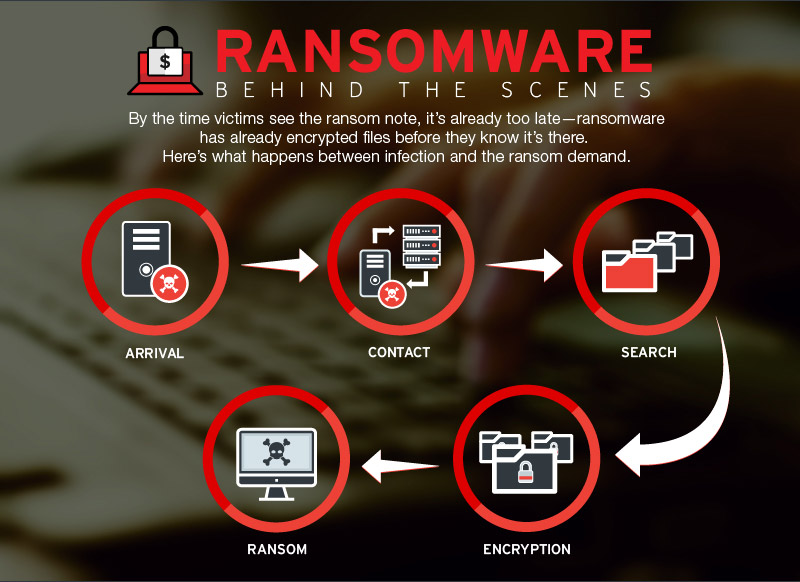
\includegraphics[scale=0.25]{./Imagenes/ransomware2.jpg}
	\pause
	\metroset{block=fill}
	\begin{block}{Esquema básico}
		\begin{itemize}
			\item Infección.
			\pause
			\item Extorsión.
			\pause
			\item Cesión.
			\pause
			\item Fraude.
		\end{itemize}
	\end{block}
\end{frame}

\begin{frame}[fragile]{Consecuencias del Ransomware}
	\centering
	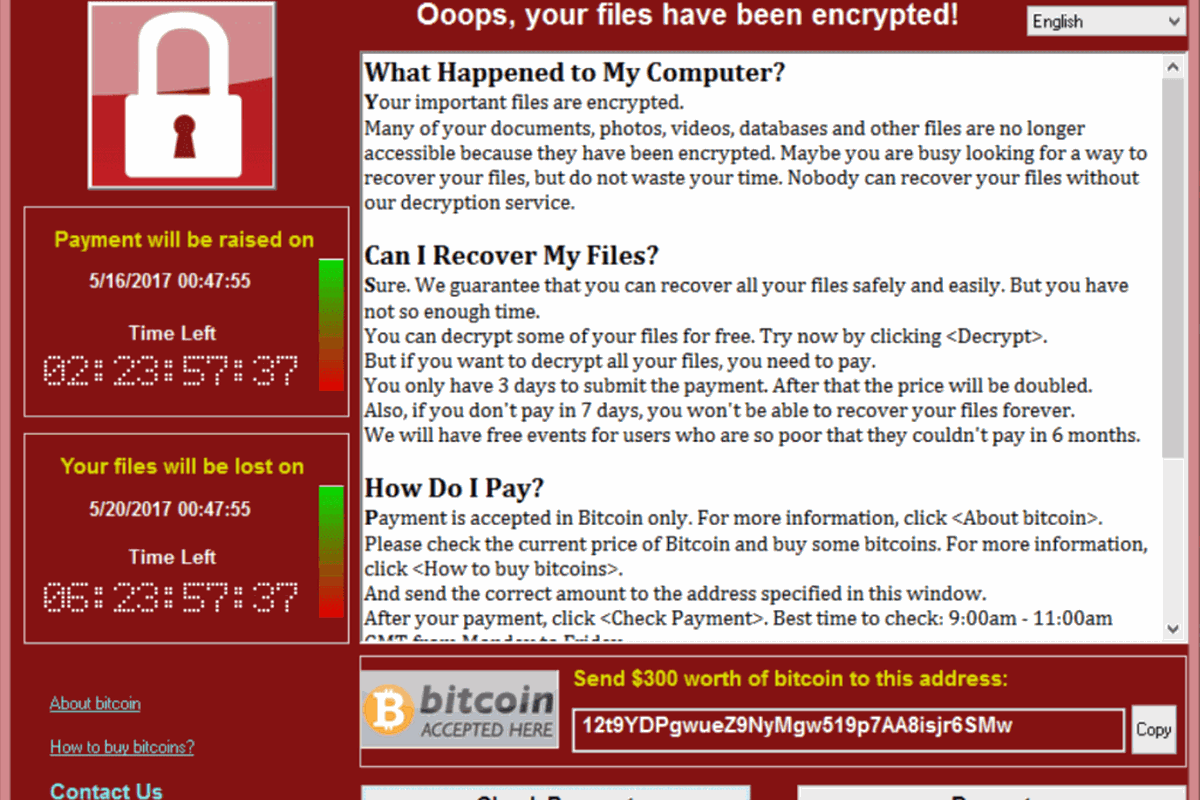
\includegraphics[scale=0.16]{./Imagenes/ransomware3.png}
	\pause
	\metroset{block=fill}
	\begin{block}{Problemas}
		\begin{itemize}
			\item Pérdida temporal o permanente de información (sensible o no sensible).
			\pause
			\item Paralización de las actividades de una empresa o persona.
			\pause
			\item Pérdidas económicas.
			\pause
			\item Denostación de la reputación de una empresa.
		\end{itemize}
	\end{block}
\end{frame}

\begin{frame}[fragile]{Vectores de infección}
	\centering
	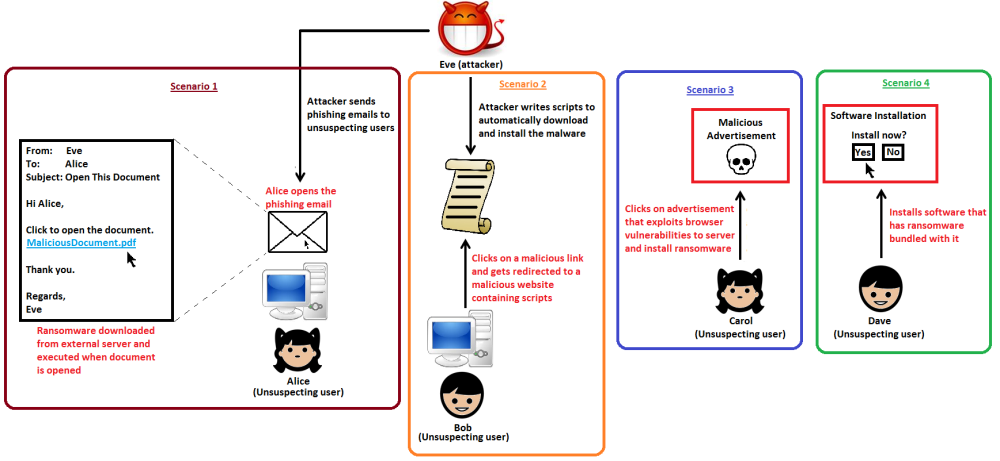
\includegraphics[scale=0.36]{./Imagenes/ransomware4.png}
	\pause
	\metroset{block=fill}
	\begin{block}{Vectores}
		\begin{itemize}
			\item Phishing
			\pause
			\item Archivo infectado.
			\pause
			\item Vulnerabilidades del sistema.
			\pause
			\item Anuncios o webs con contenido malicioso.
			\pause
			\item Ataque dirigido.
		\end{itemize}
	\end{block}
\end{frame}

\end{document}
